% TikZ figures for quantitative charts (C1-C3)
% Include this file from the main LaTeX paper.

\begin{figure}[htbp]
    \centering
    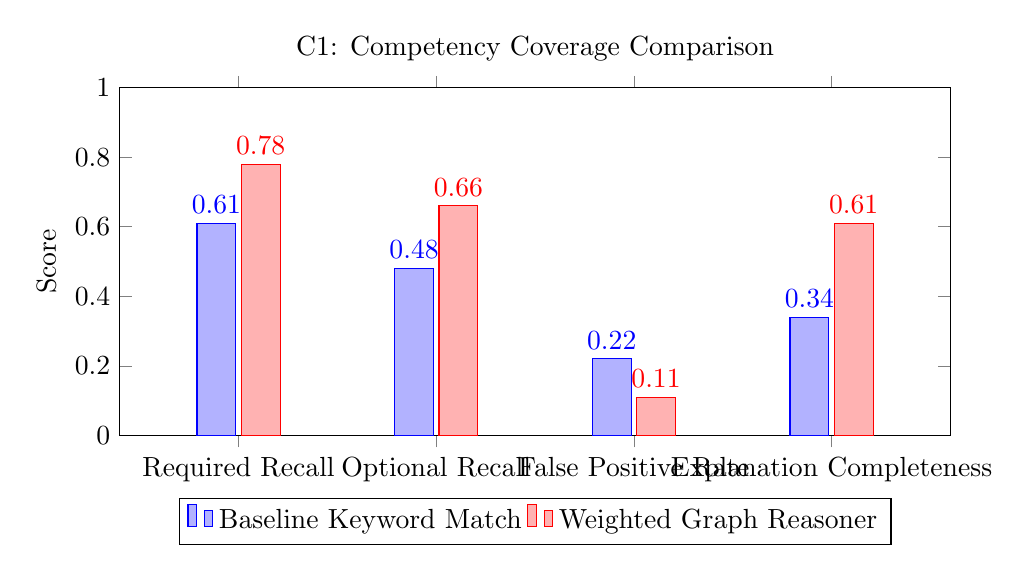
\begin{tikzpicture}
        \begin{axis}[
            ybar,
            bar width=14pt,
            width=\linewidth,
            height=6cm,
            enlarge x limits=0.2,
            ymin=0,
            ymax=1,
            ylabel={Score},
            symbolic x coords={Required Recall,Optional Recall,False Positive Rate,Explanation Completeness},
            xtick=data,
            legend style={at={(0.5,-0.18)},anchor=north,legend columns=-1},
            nodes near coords,
            nodes near coords align={vertical},
            title={C1: Competency Coverage Comparison}
        ]
        \addplot coordinates {
            (Required Recall,0.61)
            (Optional Recall,0.48)
            (False Positive Rate,0.22)
            (Explanation Completeness,0.34)
        };
        \addplot coordinates {
            (Required Recall,0.78)
            (Optional Recall,0.66)
            (False Positive Rate,0.11)
            (Explanation Completeness,0.61)
        };
        \legend{Baseline Keyword Match,Weighted Graph Reasoner}
        \end{axis}
    \end{tikzpicture}
    \caption{Competency coverage metrics comparing the legacy keyword baseline with the weighted graph reasoning engine. Lower is better for false-positive rate; higher is better for other metrics.}
    \label{fig:coverage-comparison}
\end{figure}

\begin{figure}[htbp]
    \centering
    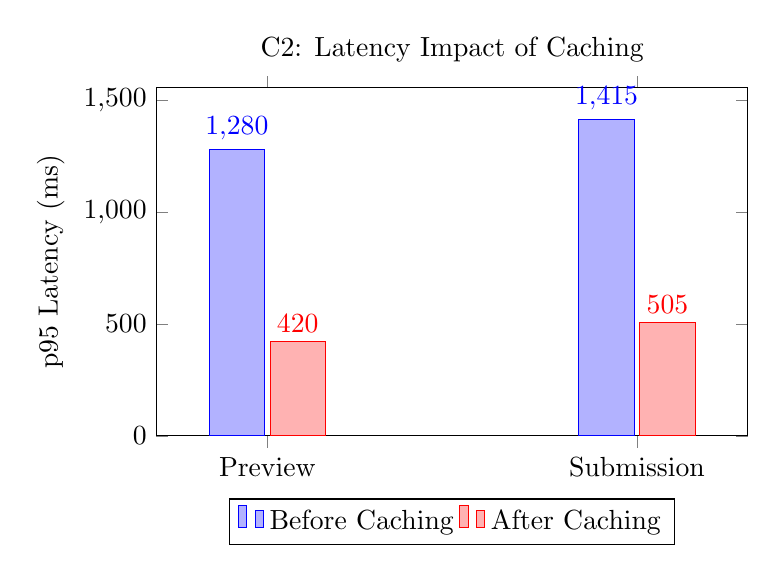
\begin{tikzpicture}
        \begin{axis}[
            ybar,
            bar width=20pt,
            width=0.75\linewidth,
            height=6cm,
            enlarge x limits=0.3,
            ymin=0,
            ylabel={p95 Latency (ms)},
            symbolic x coords={Preview,Submission},
            xtick=data,
            legend style={at={(0.5,-0.18)},anchor=north,legend columns=-1},
            nodes near coords,
            nodes near coords align={vertical},
            title={C2: Latency Impact of Caching}
        ]
        \addplot coordinates {
            (Preview,1280)
            (Submission,1415)
        };
        \addplot coordinates {
            (Preview,420)
            (Submission,505)
        };
        \legend{Before Caching,After Caching}
        \end{axis}
    \end{tikzpicture}
    \caption{Latency reductions achieved by caching for preview and submission workflows.}
    \label{fig:latency-caching}
\end{figure}

\begin{figure}[htbp]
    \centering
    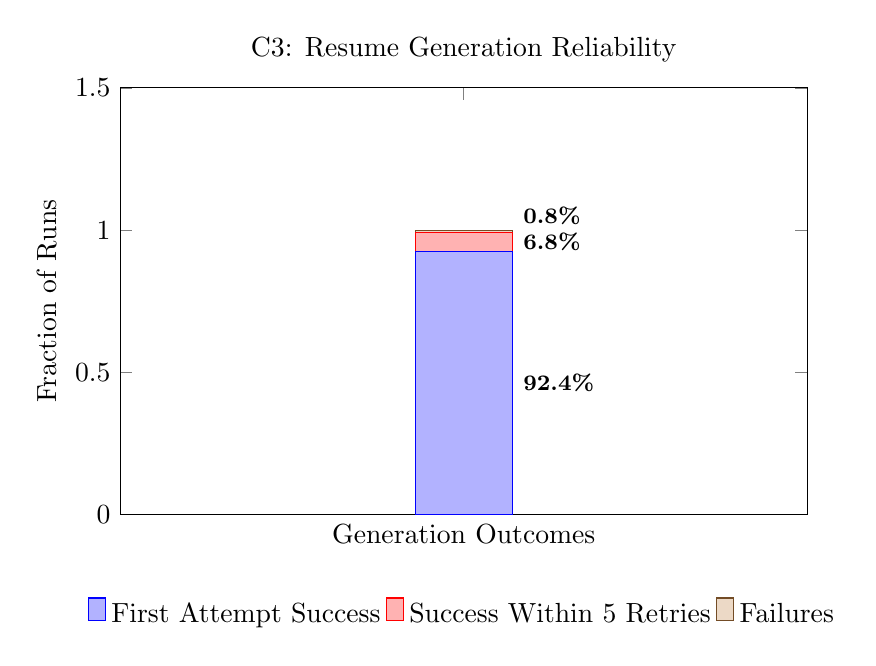
\begin{tikzpicture}
        \begin{axis}[
            ybar stacked,
            bar width=35pt,
            width=0.85\linewidth,
            height=7cm,
            enlarge x limits=1.2,
            ymin=0,
            ymax=1.5,
            ylabel={Fraction of Runs},
            symbolic x coords={Generation Outcomes},
            xtick=data,
            clip=false,
            legend style={at={(0.5,-0.18)},anchor=north,legend columns=3,draw=none},
            title={C3: Resume Generation Reliability}
        ]
        \addplot coordinates {(Generation Outcomes,0.924)};
        \addplot coordinates {(Generation Outcomes,0.068)};
        \addplot coordinates {(Generation Outcomes,0.008)};
        \legend{First Attempt Success,Success Within 5 Retries,Failures}
        \node[font=\footnotesize\bfseries,anchor=west,xshift=18pt] at (axis cs:Generation Outcomes,0.462) {92.4\%};
        \node[font=\footnotesize\bfseries,anchor=west,xshift=18pt] at (axis cs:Generation Outcomes,0.958) {6.8\%};
        \node[font=\footnotesize\bfseries,anchor=west,xshift=18pt] at (axis cs:Generation Outcomes,1.05) {0.8\%};
        \end{axis}
    \end{tikzpicture}
    \caption{Distribution of resume generation outcomes with stacked success rates. Failures encompass the remaining 0.8\% of runs.}
    \label{fig:resume-reliability}
\end{figure}
